\subsection{Polytope input language}
\label{subsec:preliminaries-polytope-input-language}

The finite methods represent polytopes by normalized halfspaces. Let
\(K\subset\mathbb R^4\) be full-dimensional with
\(0\in\operatorname{int}(K)\). We write
\begin{equation}\label{eq:preliminaries-normalized-halfspaces}
  K=\{x\in\mathbb R^4:\langle a_i,x\rangle\leq1,
    \ i=1,\ldots,F\}.
\end{equation}
If \(n_i\) is the outward unit normal to the corresponding supporting
hyperplane and \(h_i=h_K(n_i)>0\) is its height, then
\[
  a_i=\frac{n_i}{h_i}.
\]
For an irredundant description, the vectors \(a_i\) are precisely the vertices
of the polar body
\[
  K^\circ=\operatorname{conv}\{a_1,\ldots,a_F\}.
\]

\begin{figure}[htbp]
  \centering
  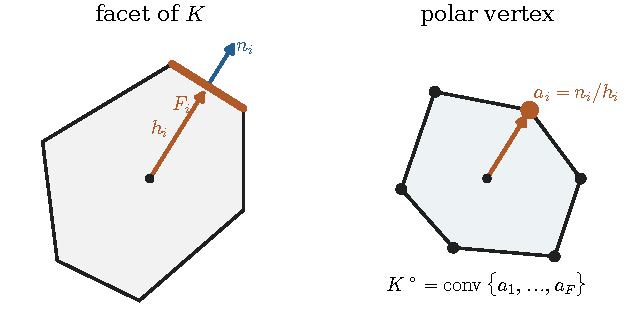
\includegraphics[width=0.92\linewidth]
    {figures/foundations/facet-polarity.pdf}
  \caption{Facet normalization and polarity in a planar model.  The
  supporting line \(\langle n_i,x\rangle=h_i\) becomes
  \(\langle a_i,x\rangle=1\) after setting \(a_i=n_i/h_i\), and that row is a
  vertex of the polar polygon.  The same facet--polar-vertex correspondence
  holds in four dimensions; the planar metric proportions are specific to
  this example and are not part of the duality statement.}
  \label{fig:preliminaries-facet-polarity}
\end{figure}

Conversely, the normalized halfspaces define a bounded full-dimensional
polytope containing the origin in its interior exactly when
\(0\in\operatorname{int}\operatorname{conv}\{a_i\}\).  The description is
irredundant exactly when the listed vectors are pairwise distinct and every
\(a_i\) is an extreme point of this convex hull.

The ordered list \((a_1,\ldots,a_F)\) is a labelled presentation.  Relabelling
the same inequalities does not change the unlabelled convex body, but labels
matter when an algorithm records facet words or when a local calculation uses
the \(a_i\) as coordinates.
